%%%%%%%%%%%%%%%%%%%%%%%%%%%%%%%%%%%%%%%%%%%%%%%%%%%%%%%%%%%%%%%%%%%
%                                                                 %
%                            CHAPTER FIVE                         %
%                                                                 %
%%%%%%%%%%%%%%%%%%%%%%%%%%%%%%%%%%%%%%%%%%%%%%%%%%%%%%%%%%%%%%%%%%%

\chapter{DETERMINING DATA VOLATILITY} \label{Volatility}

\section{Introduction}

\Glspl{changedist} opens new avenues to study and communicate data set change beyond the surface analysis provided by version labeling.
The bar graph in Figure \ref{GCMDC1} showing the amount of change in each \gls{gcmd} version release only shows the relation of the \glspl{change} to each \gls{version} and disconnects the \glspl{change} from time.
The bar graph presents a flawed view because the evenly spaced bars imply the distance, in time, between \gls{version} releases are the same.
Such a view of how the \glspl{version} are released suggests that not only is the \gls{changedist} between \glspl{version} large, but that the change rate is also large.
The change rate communicates expectations for the data consumer on the value of a data set since committing to a data set that will soon be invalidated is problematic.
The following chapter addresses data \gls{volatility}, the likelihood of data change, and  how traditional \glspl{version} can hide the actual change rate of data sets.

\section{Determining Volatility}

Instead of charting the \gls{version} \glspl{change} in evenly wide bars, the \glspl{version} are spread across time based on the time of publication to the \gls{kms} as seen in Figure \ref{GCMDPlot1}.
\begin{figure}%[b]
	\centering
	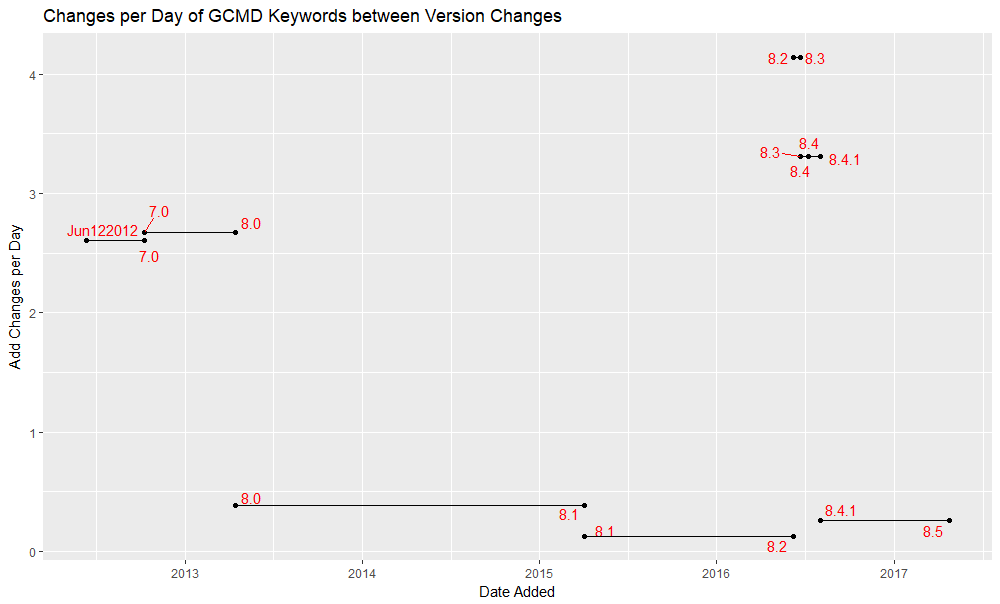
\includegraphics[scale=0.56]{figures/GCMDPlot1.png}
	\caption[Global Change Master Direcotry counts distributed over time.]{Add counts for all versions of GCMD up to 8.5 evenly distributed over the time of version validity.}
	\label{GCMDPlot1}
\end{figure}
Since each of the \glspl{version} were dominated by the \gls{add} counts, the count is divided by the number of days between the publication of a \gls{version} on the left side of the line and the release of the replacement \gls{version} on the right side of the line.
The height of the line on the chart gives the amortized rate of change until the release of the new version.
The area underneath the line is the total amount of change the new \gls{version} introduces.
Since each \gls{version} packages together all the \glspl{change} into a single release, the actual change rate is unknown.

Three observable clusters appear in the time aware presentation of the \glspl{version}, highlighted in Figure \ref{GCMDPlot1Cluster}.
\begin{figure}%[b]
	\centering
	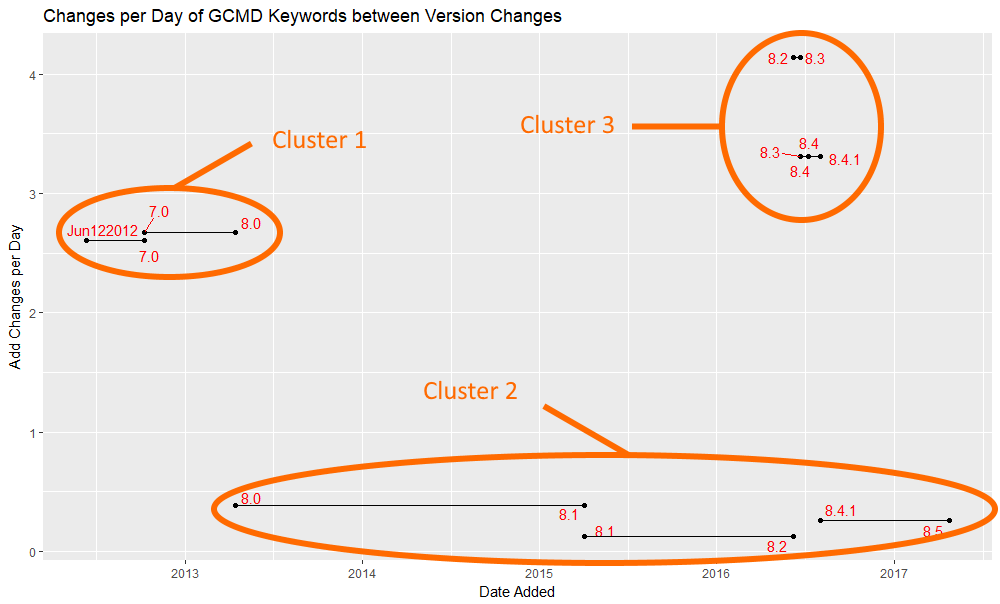
\includegraphics[scale=0.56]{figures/GCMDPlot1_Cluster.png}
	\caption[Global Change Master Directory count distributed over time with clusters marked.]{The change rate of different Global Change Master Directory versions organized into three visible clusters. Cluster 2 denotes a sudden burst of version releases which is notable.}
	\label{GCMDPlot1Cluster}
\end{figure}
According to the \textit{Keyword Governance and Community Guide Document} \cite{gcmd_gov}, ``Full GCMD keywords list releases get a new major version number (e.g., 8.0). Incremental releases for updates to topics, terms, and variables get a new minor version number (e.g., 8.1).”
The statement explains the activity in Cluster 1 where there are sufficient \glspl{change} to warrant a full release of the keywords.
Cluster 2 captures the change rate and duration of minor versions, except those from 8.2 to 8.4.1 which are in Cluster 3.
Cluster 3 demonstrates a flurry of activity occurring between June 7, 2016, to August 2, 2016.
Considering the previous pattern of taking at least six months between releases, three minor version releases within as many months is highly unusual.

An immediate concern is that Cluster 3 does not result from a sudden burst of activity, necessitating rapid \gls{version} replacement.
An email inquiry (T. Stevens, personal communication, May 2, 2018) into reasoning behind the successive publication returned a statement that ``Our government customer had directed us to release the keywords all at once this way."
Another way to dig into the behavior is to look into the impact assessments accompanying the versions.
Impact assessments prior to Version 8.5 are not publicly available, and only assessments for versions 8.2, 8.3, and 8.4 were received upon request.
Of the 6 requests affecting Earth Science Keywords in 8.2, published June 7, 2016, 4 were made in 2014, and the remaining 2 were made in 2015.
Version 8.3 had 8 entries in its impact assessment with 7 entries originating in 2014, and the remaining entry from 2015.
The 6 entries 8.4’s impact assessment has 5 entries from 2008 and 1 entry from 2015.
The data is collected in Table \ref{table:GCMD_old}.
\begin{table}
	\caption{Global Change Master Directory versions with old start time changes.}
	\label{table:GCMD_old}
	\centering
	\begin{tabular}{|c|c|c|c|c|}
		\hline
		Version Name&	Publish Date&	2008&	2014&	2015\\ \hline
		8.2&	June 7, 2016&	0&	4&	2\\
		8.3&	June 21, 2016&	0&	7&	1\\
		8.4&	July 7, 2016&	5&	0&	1\\
		\hline
	\end{tabular}
\end{table}


\section{Earth Observing Laboratory}

The \gls{eol} of the \gls{ncar} distributes small data sets, around 10-12 files per data set, regarding lower atmospheric data beginning in 2005 \cite{EOL}.
The \gls{eol} data sets are unique in the data set size means management often does not require automation.
In mid-2014, \gls{eol} began assigning \gls{version} to stored data sets.
When receiving a new \gls{version} of a data set from a researcher, the practice is to upload the entire new data set, and replace all old files.

The meta-data extraction and analysis was done by the script found in Appendix \ref{app:eol}.
The script organizes the information into classes representing the data set, the versions of the data set, and the files within the versions.
The nested class structure allows federated data computation by having each data set manage version analysis within the data set object.
The versions also become grouped and co-located with associated versions in the same data set.

Of the 1335 data sets maintained by \gls{eol} with \glspl{version}, only 180 data sets had more than one \gls{version}.  
The full distribution of version counts is in Table \ref{table:EOL_Versions}
\begin{table}
	\caption{Version Aggregate of Earth Observing Laboratory Data Sets}
	\label{table:EOL_Versions}
	\centering
	\begin{tabular}{|c|c|}
		\hline
		Number of Versions& Number of Data Sets\\ \hline
		1&	1155\\
		2&	141\\
		3&	26\\
		4&	10\\
		5&	3\\ \hline
		Total&	1335\\
		\hline
	\end{tabular}
\end{table}
The 1155 other data sets were filtered out since \gls{changedist} could not be computed for single-version collections.
Since all the files are replaced on an update and a unique file identifier like a hash sum was unavailable, file matching between versions rely on filenames to perform change mappings.
For all files that matched names across \glspl{version}, the relation was classified as \gls{modify}.  
This approach will over-count the number of \glspl{modify}, but provides an upper bound on the data set \gls{volatility} in the repository.  
Each count is then normalized by the number of files in the previous \gls{version} to standardize comparison between data sets regardless of data set size.  
The average for each data set is taken for each \gls{AIM} \gls{change}.

\subsection{EOL Versioning Behavior} \label{sec:behavior}

Given that \gls{eol} replaces the entire old data set when updating, the expected behavior of the transitions would be \glspl{modify} concentrating close to 1 and \glspl{add} and \glspl{invalidate} distributed close to 0.
The assumption is that researchers have little reason to change the file naming scheme.
The data surprisingly indicates that data sets in \gls{eol} primarily gravitate towards \gls{add} and \gls{invalidate} values of 1.
\gls{modify} counts score more close to 0 in a complete reversal of expectations.

Figure \ref{EOL_Adds} shows the distribution of \gls{add} scores.
\begin{figure}%[b]
	\centering
	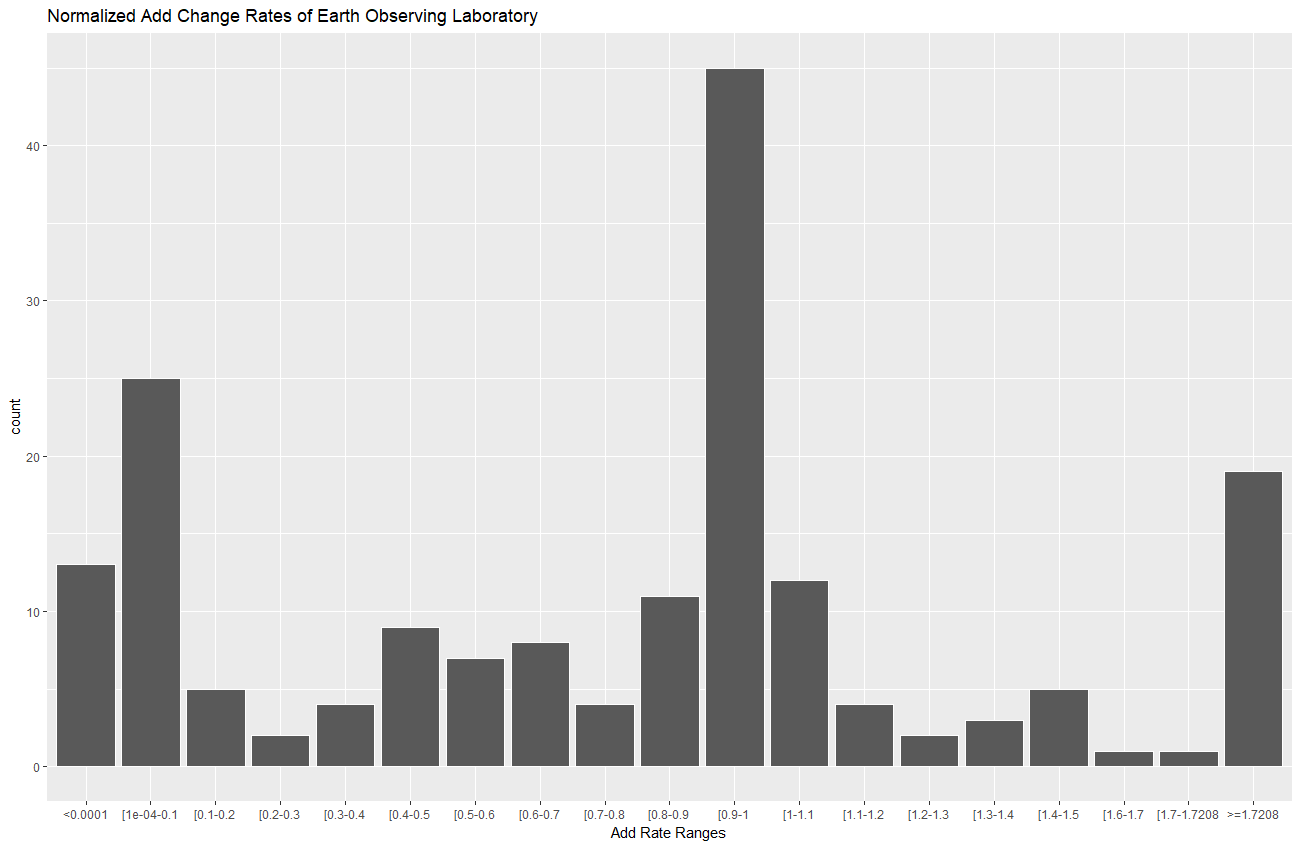
\includegraphics[scale=.43]{figures/Eol_Adds.png}
	\caption{Distribution of average normalized Add counts for each data set in Eath Observing Laboratory.}
	\label{EOL_Adds}
\end{figure}
The primary feature of the chart is the bar situated in the `[0.9-1' range, meaning that about 45 data sets add a number of files equal to the original size of the data set.
Secondary features include the bars on the far right and far left of the chart, but the bar on the right side is a collection of outliers.
In the outlier data sets, the size of the data set increased drastically compared to the behavior of other data sets managed by \gls{eol}.
Outliers are determined by collecting values above 1.5 times the \gls{iqr} showing in Table \ref{table:EOL_Change}.
\begin{table}
	\caption{Normalized Change Statistics}
	\label{table:EOL_Change}
	\centering
	\begin{tabular}{|c|c|c|c|}
		\hline
		Stat&	Add&	Invalidate&	Modify\\ \hline
		Mean&	0.714312707&	0.654819294&	0.345180706\\
		Std. Dev&	0.509878564&	0.420093557&	0.420093557\\
		Min&	0&	0&	0\\
		Q1&	0.28635075&	0.142857&	0\\
		Med&	0.9146635&	0.9642855&	0.0357145\\
		Q3&	1.00358625&	1&	0.857143\\
		Max&	54.25&	1&	1\\
		IQR&	0.7172355&	0.857143&	0.857143\\
		\hline
	\end{tabular}
\end{table}
A more muted distribution appears around the 0.5 mark where data sets grow more gradually.

The normalized \gls{invalidate} score in Figure \ref{EOL_Invs} shows a majority of data sets removing all or almost all files in the data set.
\begin{figure}%[b]
	\centering
	\includegraphics[scale=.6]{figures/Eol_Inv.png}
	\caption{Distribution of average normalized Invalidate counts for each data set in Eath Observing Laboratory.}
	\label{EOL_Invs}
\end{figure}
Coupled with the information that a quarter of the data sets added close to the original data sets' size of files suggests that the entire data set is being replaced.
\Glspl{invalidate} do not have outliers since only files within the data set can be removed.
The \gls{invalidate} distribution is extremely biased with only 0.04 separating the median and maximum value.
From Table \ref{table:EOL_Change}, at least a quarter of values are 1.
Figure \ref{EOL_Invs} also shows a muted distrubtion around 0.5.

Figure \ref{EOL_Mods}, representing the normalized \gls{modify} distribution, is almost a mirror of the \gls{invalidate} chart.
\begin{figure}%[b]
	\centering
	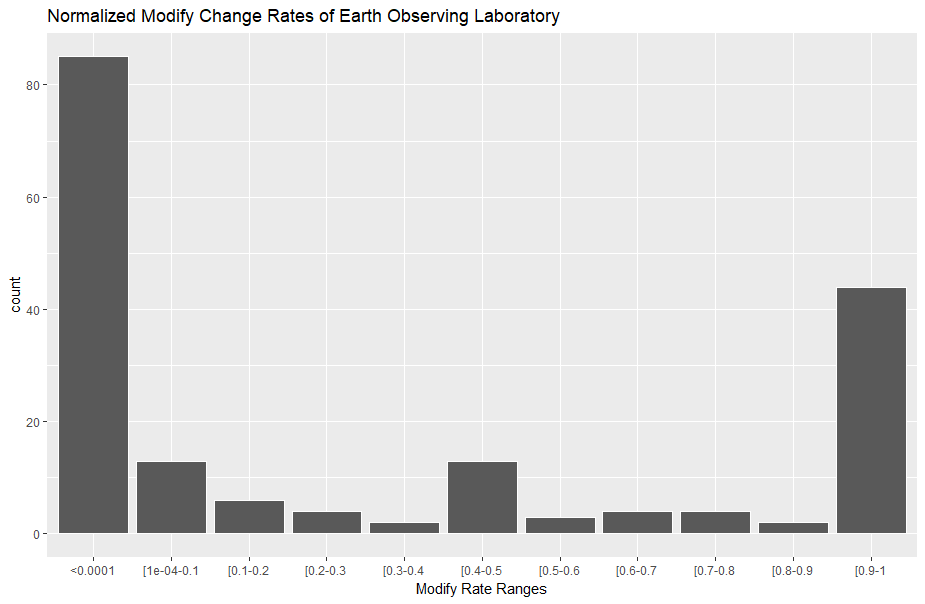
\includegraphics[scale=.6]{figures/Eol_Mod.png}
	\caption{Distribution of average normalized Modify counts of each data set in Eath Observing Laboratory.}
	\label{EOL_Mods}
\end{figure}
The right bar is specifically cut off to capture only 0s, showing that almost a majority of data sets modify 0 files, having 0 files that share names between \glspl{version}.
The distribution is consistent with a practice of removing all the files in a data set and replacing the files with a new data set using different filenames.
The second feature of this graph shows around 40 data sets in which all or almost all files match across \glspl{version}.
A small spike of data sets are centralized around 0.5, very much like the other normalized change graphs.

The high concentration of data sets towards 1 in \glspl{add} and \glspl{invalidate} suggests a more complicated interaction within the data sets.
Individually, the normalized distributions do not show the connection between all three changes since the \glspl{change} share a common feature, the version transition the \glspl{change} describe.
Together, the \gls{AIM} \glspl{change} create a coordinate in three dimensional space, showing the inter-relation of the \glspl{change}. 
Figure \ref{EOL_AIM} shows a scatter plot grouping unnormalized \glspl{changedist} for each \gls{version}.
\begin{figure}%[b]
	\centering
	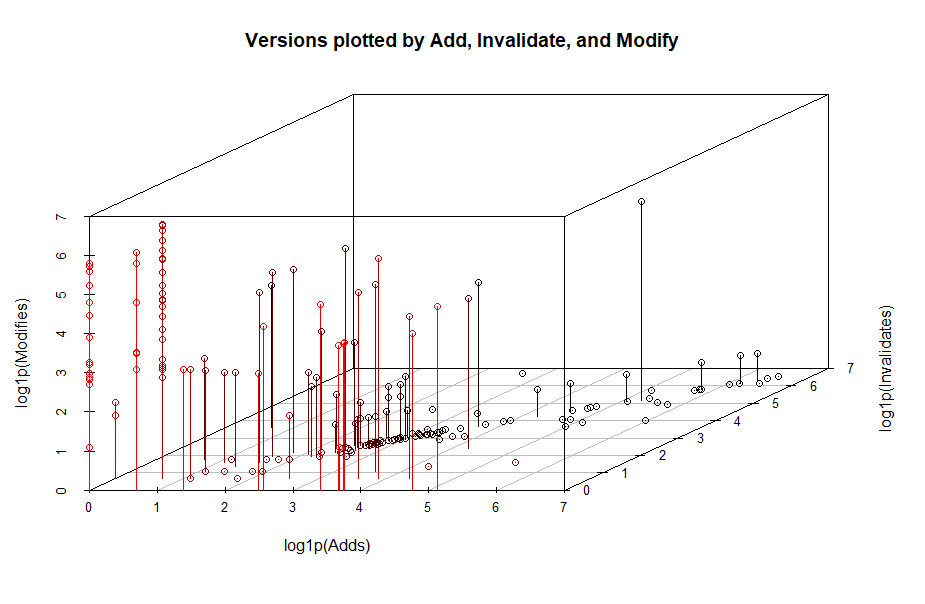
\includegraphics[scale=.6]{figures/Eol_Versions_3d.png}
	\caption{Versions in the Earth Observing Laboratory data collection plotted as a combination of \textbf{Add}, \textbf{Invalidate}, and \textbf{Modify} counts.}
	\label{EOL_AIM}
\end{figure}
Unlike the other charts, the size of the changes are not normalized by data set size, but the values have the log1p function applied to account for a heavy bias towards 12 and 13.
Notice the one-to-one trend between \glspl{add} and \glspl{invalidate} which shows the tendency of data sets to replace every file and assign a new filename.
If the two \glspl{change} did not co-occur, a normalized \gls{add} score of 1 would indicate that data sets tend to double in size instead.
The files are more likely to retain filenames when only a few files in a data set are being modified.

\section{Analysis}

\subsection{Impact Assessment Change Counts}

The impact assessments obtained for \gls{gcmd} Version 8.2, 8.3, and 8.4 revealed that some of the \glspl{change} began much earlier than the valid duration of the previous \gls{version}.
Adjusting for the new duration, the change rates reduce to under 0.5, aligning with the values in Cluster 2 in Figure \ref{GCMDPlot1Cluster}.
The impact assessments furthermore provide change counts in the format of \gls{add}, \gls{invalidate}, and \gls{modify}.
In none of the cases, shown in Table \ref{table:GCMD_metric}, did the metrics completely align although Version 8.3 came close with a difference of 3.
\begin{table}
	\caption{Differences in VersOn and Impact Assessment metrics}
	\label{table:GCMD_metric}
	\centering
	\begin{tabular}{|r|r|r|r|}
		\hline
		Version & Add & Invalidate & Modify\\ \hline
		8.2(VO)&	53&	1&	26\\
		-8.2(IA)&	48&	0&	4\\
		\hline
		&	\textbf{5}&	\textbf{1}&	\textbf{22}\\
		\hline
		8.3(VO)&	58&	0&	13\\
		-8.3(IA)&	58&	0&	10\\
		\hline
		&	\textbf{0}&	\textbf{0}&	\textbf{3}\\
		\hline
		8.4(VO)&	53&	0&	1\\
		-8.4(IA)&	66&	0&	5\\
		\hline
		&	\textbf{-13}&	\textbf{0}&	\textbf{-4}\\
		\hline
		8.5(VO)&	68&	2&	22\\
		-8.5(IA)&	55&	0&	30\\
		\hline
		&	\textbf{13}&	\textbf{2}&	\textbf{-8}\\						
		\hline
	\end{tabular}
\end{table}
\gls{vo} does not consistently overestimate or underestimate across the \glspl{version}, but the assessments most consistently align on \gls{invalidate} which make up very few of the \glspl{change}.

An investigation into the specific differences in Version 8.3 revealed that the term ``Saline Lake" does not appear in the \gls{log}, but ``Leaf Area Index (LAI)" appears twice.
LAI appears twice because it has two unique identifiers.
Six terms appeared in the \gls{log} as \gls{modify} but missed three terms from the impact assessment.
The primary driver between the differences lies in impact assessments being sourced from community requests.
The focus of the change analysis becomes arranged around the preferred label rather than the unique identifier used to implement the keyword.
Impact assessments capture changes that modify a keyword's label and that doesn't change the keyword's place in the taxonomy as a result.
The \gls{log} uses a keyword's unique identifier and its placement in the taxonomy to determine changes to the structure.
The difference in metrics collection once again illustrates the producer/consumer dynamic in data version management as well as the need for clear versioning practices.
While the comparison between the two counts would be invalid due to differences in practice, a valid comparison could be constructed using the unique identifier to align entries and just the preferred label to determine if the keywords differ.

\subsection{Hidden Volatility}

To determine if the actual change rate is being obscured by the version publication rate, the duration of each \gls{version} must be calculated.
Since only one \gls{version} is published at the end of that duration, simply taking the inverse of the duration will give the version publication rate.
The change counts are then multiplied by the version publication rate for each \gls{version} to acquire the change rate for each \gls{version}.
Because the \glspl{changedist} are often the size of the data sets, as shown in Figure \ref{EOL_AIM}, the means must be adjusted to align with the version publication rate mean in order to perform the Kolmogorov-Smirnov test.
The test will determine the likelihood that the change distribution comes from the same distribution that produced the version publication rates.

Each \gls{version} of a data set stored in \gls{eol} is assigned three different times, ``version publish time," ``version creation time," and ``version modification time." 
Version publish time indicates the time the \gls{version} was made available to the public, usually the data set was added to the database.  
Version creation time denotes the moment at which a \gls{version} designation was given to the collection of files, beginning in mid-2014 when the versioning system was implemented.  
Version modification time indicates the time at which the \gls{version} metadata was changed.  
Using version publish time most closely resembles the duration of version validity, and the following computations use version publish time.

\begin{table}
	\caption{Summary of Kolmogorov-Smirnov Test results for Earth Observing Laboratory.}
	\label{table:Eol_KS}
	\centering
	\begin{tabular}{|c|c|c|c|c|}
		\hline
		&	Add&	Invalidate&	Modify&	Versions\\ \hline
		Length&	205&	192&	114&	227\\
		D-Value&	0.12919&	0.14464&	0.19727&	NA\\
		p-Value&	0.05487&	0.02575&	0.005443&	NA\\
		\hline
	\end{tabular}
\end{table}
The duration is calculated by taking the publish time of the next \gls{version} and subtracting the publish time of the current \gls{version}.
Some of the durations needed to be filtered out to provide valid results.  
Due to a few coding errors in time assignments, 7 \glspl{version} had to be removed because the durations were negative.  
\begin{figure}
	\centering
	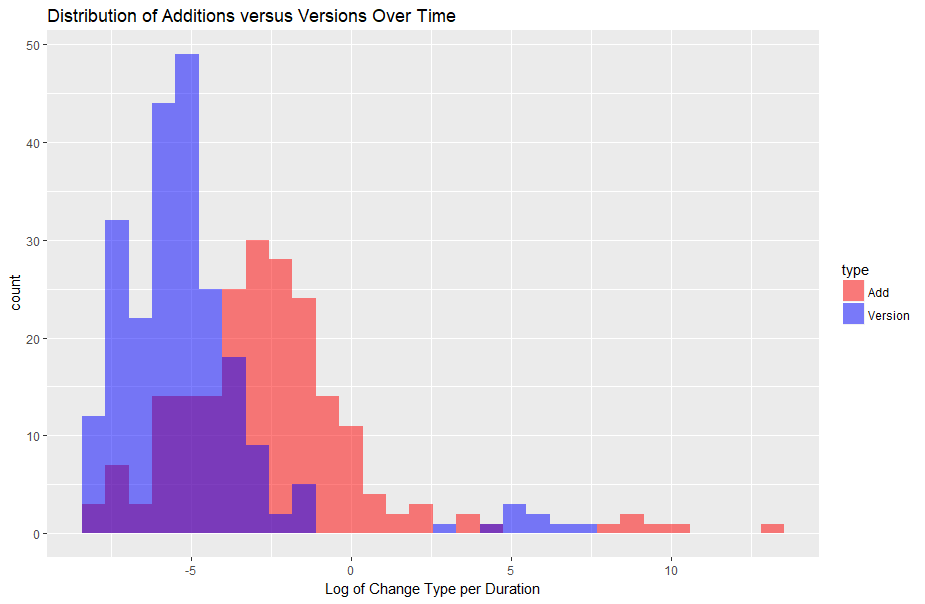
\includegraphics[scale=.5]{figures/Eol_Add_Ver_Rate.png}
	\caption{Distribution of \textbf{Add} rates of each version against the version publication rate in Earth Observing Laboratory.}
	\label{EOL_Add_Ver}
\end{figure}
\begin{figure}%[b]
	\centering
	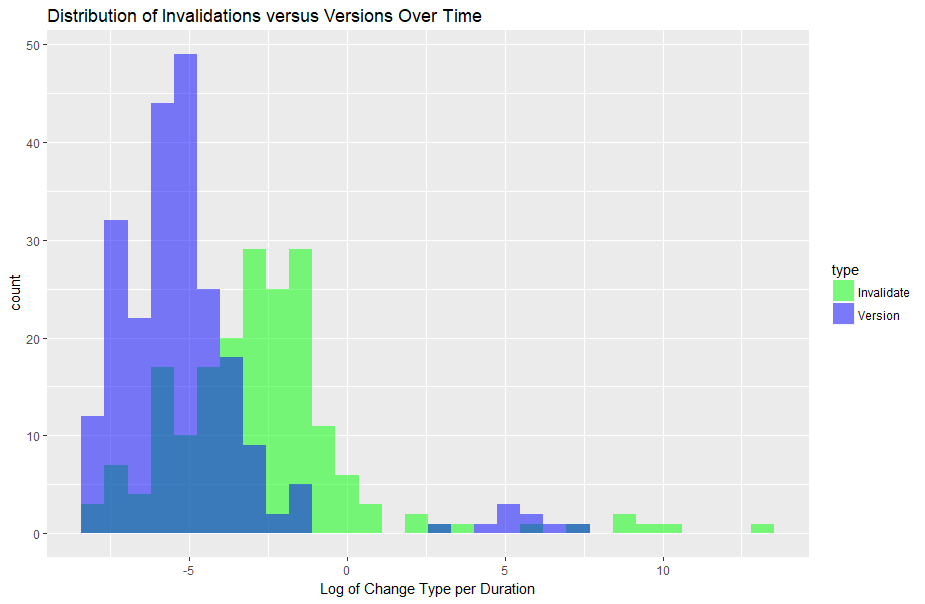
\includegraphics[scale=.5]{figures/Eol_Inv_Ver_Rate.png}
	\caption{Distribution of \textbf{Invalidate} rate of each version against the version publication rate set in Eath Observing Laboratory.}
	\label{EOL_Inv_Ver}
\end{figure}
Duration is measured in days, and the rate of version publication is determined by taking the inverse of the duration, giving versions per day.  
To acquire the \gls{AIM} change rates, the \glspl{change} are divided by the associated duration for each \gls{version}, returning change per day.  
Since the change rates are biased towards 0, the log of the rates are taken to give the values a more normal distribution.  
Values where an \gls{AIM} change is 0 had to be removed in order to properly apply the log function.  
The size of each distribution can be found in Table \ref{table:Eol_KS}.

Since the durations are log-normally distributed, concentrated close to 0, the log of the durations are taken to normalize the data.  
The log function is also applied to the \gls{AIM} changes after the division by the duration.  
The inverse of the log of the duration is taken to acquire the rate of \gls{version} release.
The \gls{add} distribution in Figure \ref{EOL_Add_Ver} and the \gls{invalidate} distribution in Figure \ref{EOL_Inv_Ver} are translated slightly a few points to the right of the darker \gls{version} distribution.
As noted in Section \ref{sec:behavior}, almost half of the \glspl{version} have 0 \glspl{modify}, meaning that the values must be filtered out.
The resulting graph for comparison in Figure \ref{EOL_Mod_Ver} shows a more flattened \gls{modify} distribution.
\begin{figure}[b]
	\centering
	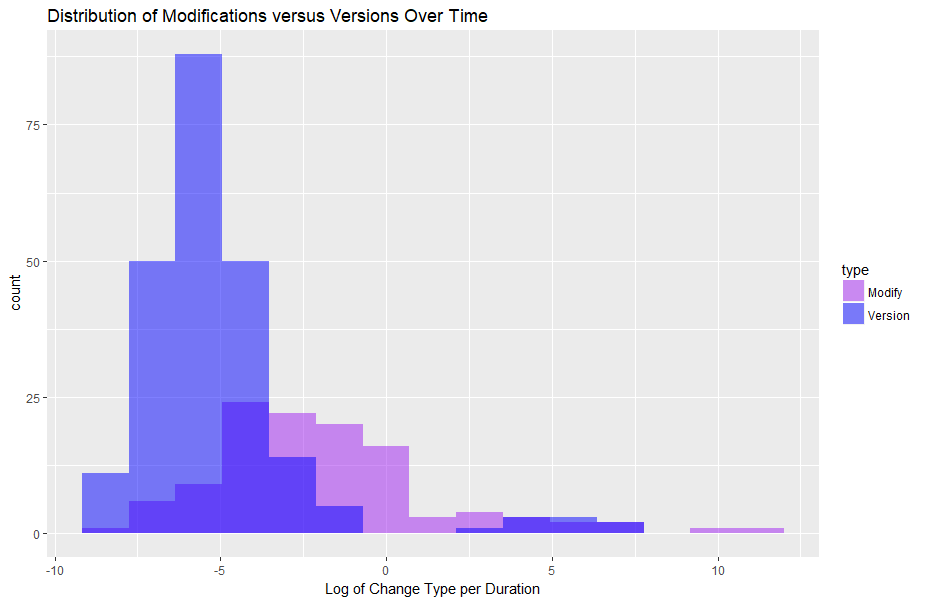
\includegraphics[scale=.6]{figures/Eol_Mod_Ver_Rate.png}
	\caption{Distribution of average normalized Modify counts of each data set in Eath Observing Laboratory.}
	\label{EOL_Mod_Ver}
\end{figure}

The Kolomogorov-Smirnov Test was used to determine if the \glspl{add}, \glspl{invalidate}, or \glspl{modify} follow a distribution the same as the version publication distribution as the null hypothesis.  
The change distributions were translated down such that the \gls{version} mean and the \gls{change} mean aligned in order for the test to produce meaningful results.
Table \ref{table:Eol_KS} shows that the distribution of \glspl{add} is statistically significant with 90\% confidence while \glspl{invalidate} and \glspl{modify} can reject the null hypothesis with at least 95\% confidence.
The analysis demonstrates that there is strong evidence version publications do not accurately reflect the actual change rate of the \gls{eol} data sets.

Overlaying the change distributions in Figure \ref{EOL_AIM_Rate}, notice the distributions are all log-normally distributed around the same mean.
\begin{figure}%[b]
	\centering
	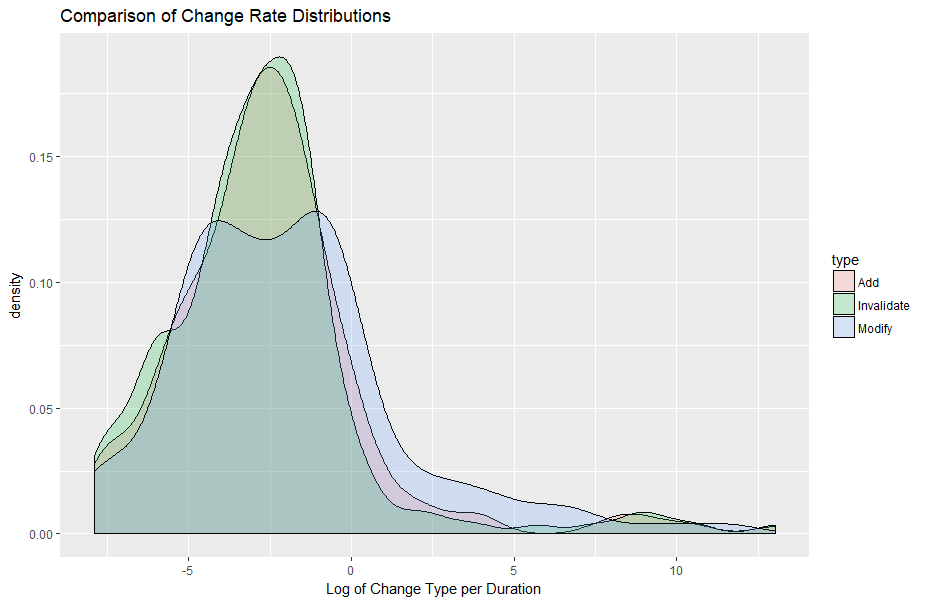
\includegraphics[scale=.6]{figures/Eol_AIM_Rate.png}
	\caption[Density plot of change rates in Eath Observing Laboratory divided by type.]{Density plot of change rates in Eath Observing Laboratory divided by type.}
	\label{EOL_AIM_Rate}
\end{figure}
The normality indicates that data users can reliably predict the rate of \gls{add} or \gls{invalidate} for a data set, setting an expectation for the valid duration of a \gls{version} the data consumer currently uses.
The distribution additionally allows a data consumer to predict an expected amount of \gls{change} in a data set after not updating the data for a period of time.
The flatter \gls{modify} density curve shows a bi-modal behavior, suggesting that \gls{modify} changes follow two separate distributions.
Remember that the \gls{modify} counts reflect an upper-bound value of \gls{change} in \glspl{version} and many data sets completely replace the files in a \gls{version}.
The two distributions likely reflect the behavior of \glspl{version} of differing maturity with older versions of data sets requiring fewer modifications to the data, resulting in a lower change rate.
Drawing expectations from Figure \ref{EOL_AIM_Rate} should be done carefully since Section \ref{sec:behavior} shows that \gls{modify} does not correlate the same way that \gls{add} and \gls{invalidate} do.
The different behavior means that the change rates are not independent distributions.

\section{Summary}

Implementing the versioning model, \gls{vo}, yielded results more complicated than the simple model expected.
While \gls{vo} addresses difficulties in other linked data approaches, it requires many more triples to express the relationship.
The scalability created space issues with encoded \glspl{log}, especially in \gls{jsonld}.
\gls{rdfa} also proved to be a more restrictive structured data method than expected.
The implementation required multiple attributes per \gls{modify} to accommodate both row and column \gls{attribute} associating with a cell.
There were discrepancies between \gls{gcmd} Keyword version identifiers and the change detected within the data set.
Finally, the versioning model was used not to document sequential \glspl{version}, but to compare the results of different species classifiers.

\subsection{Model}

The versioning model's development began with an expectation that versions would be sequential.
The \gls{mbvl} data set demonstrated a case where four data sets were not related by temporal sequence.
One is not a transformation of another since we are studying the effects of changing the taxonomy or algorithm.
Additionally, since we do not know which \gls{version} is the best, we cannot consider any data set as an update of the others.
Finally, no entity preexisted as the data sets resulted from an ongoing analysis and further steps have not been developed.
As a result, the current definition of \textit{prov:wasDerivedFrom} would not be able to capture the relationship between these data sets.
\gls{vo} improves upon expressing \glspl{version} in \gls{linked} by focusing on the differences between objects rather than the sequence.
\gls{vo} takes inspiration from \textit{schema:UpdateAction} by dividing up the \glspl{change} into three forms, but improves upon it by adopting the provenance model's transition from one object to the next.
The resulting forms diverge from Schema.org's context of an agent acting upon an object.

The reason \textit{prov:Generation} and \textit{prov:Invalidation} are not used is because they expect an activity to act upon an object.
It is not generally true that an action actively adds or removes an object's \gls{attribute} from in the left-hand \gls{version} to produce the right-hand \gls{version}.
That assumption minimizes the ability to conduct versioning comparisons between objects that are not sequentially adjacent.
The \gls{prov} concepts also have a property pointing towards the responsible activity which is assumed to be the immediately preceding activity.
The assumption fails to consider the case where a \gls{change} propagates further \glspl{change} downstream, generating or invalidating the current object.
\gls{vo} avoids confusion by only considering the \glspl{version} and their differences.

\subsection{Implementation}

\subsubsection{Scalability}

\gls{vo} breaks up a revision into constituent changes, acting upon different \glspl{attribute} of the \gls{version}.
Other ontologies use a single property to relate \glspl{version}.
While it is more specific, the \gls{vo} implementation encounters scalable space consumption problems.
\gls{prov} only requires 3 to 5 triples in order to make a \textit{prov:wasRevisionOf} statement.
This model uses 9 triples for a \textit{vo:ModifyChange} and 7 to encode \textit{vo:AddChange} and \textit{vo:InvalidateChange}.
An implementation of the model, therefore, has space complexity of \[O(7M+5(A+I))\] since declaring \gls{version} objects takes a constant two statements.
However, a similar structure can be achieved using \textit{prov:wasDerivedFrom} to replace modifications and \textit{schema:AddAction} and \textit{schema:DeleteAction} to replace \glspl{add} and \glspl{invalidate}.
The resulting space complexity is: \[O(7M+3A+5I)\]
This is fairly similar with \glspl{add} seeing a reduction since the left-hand \gls{version} no longer contributes to the \textit{schema:AddAction}.
Thus the primary benefit of using this model comes from semantics.

\subsubsection{Structured Data and the Model}

While machine-readable \glspl{log} have always been a desired goal of this dissertation work, their requirements diverged from the versioning model's needs.
The model, as a result, leverages very little from visible content on the \gls{log}.
Symmetric representation in the \gls{log} also made encoding the \gls{vergraph} using \gls{rdfa} challenging without explicitly defining the whole \gls{vergraph} in invisible span tags.
Adherence with a \gls{log} oriented approach would also likely have reduced the number of statements needed to form the \gls{vergraph}.
The resulting ontology would likely be a collection of properties and concepts to use in annotating a document.

The \gls{vo} construction provides great flexibility for \gls{version} and \gls{changedist} capture.
\gls{vo} adapts to multiple \glspl{attribute} smoothly.
Greater adherence to structured data adoption may need to come in the form of graph simplification or metered release of new editions to ensure that \glspl{log} do not grow too large.

\subsection{Distance Measure}

As mentioned in Section \ref{sec:usecase}, a version model provides the framework, provenance models provide the context, and \glspl{log} fill in the gap between \glspl{version}.
\glspl{log}, therefore, provide the most substance to quantify the distance between \gls{version}.
The automated \gls{log} generation additionally ensures this by including all differences into the \gls{log}.
Anything unmapped remains the same between \glspl{version} and does not contribute towards the distance.
While \gls{mbvl} demonstrated a case where domain knowledge could be added to the \gls{vergraph} and provide context for distances, other applications may not demonstrate the same amount of uniformity within changes.
More domain information and reasoning may be necessary to determine if one \gls{add} significantly more impactful than others in a \gls{vergraph}.


\subsection{Volatility}

In Chapter \ref{Volatility}, we explored different ways in which \glspl{version} hide the actual \gls{change} behavior within a data system.
The \gls{gcmd} keywords showed one perspective when evenly distributed, but spread across time, the \glspl{version} have very different behavior.
The change rates, once re-coupled to time, show that \glspl{version} can provide a misleading view of how changes apply to a data set.
\glspl{version} package together \glspl{change} that can originate from times prior to the previous \gls{version}, disrupting the assumed relationship between consecutive \glspl{version}.
\gls{gcmd} also breaks assumptions when the impact assessments use different metrics to determine a data set change, reinforcing the concept that perspective and context play a major role in versioning methodology.
Using only \gls{version} names, \gls{eol} data is distributed uniformly by single \glspl{version}, but \ref{EOL_AIM} shows a more vibrant behavior in the data sets.
The chart revealed trends in file naming and replacement.
The data sets also demonstrated that \gls{AIM} changes behave significantly differently than the behavior \glspl{version} reveal.